\documentclass{article}
\usepackage{graphicx} % Required for inserting images
\usepackage{multirow}
\usepackage{scalefnt}
\usepackage{ulem}
\usepackage{tikz}
\usepackage{pgfplots}
\usetikzlibrary{calc}
\usepackage{xfp}
\usepackage{pgfmath}
\usepackage[section]{placeins}
\usepackage{placeins}
\tikzset{caption/.style={insert path={
let \p1=($(current bounding box.east)-(current bounding box.west)$) in
(current bounding box.south) node[below,text width=\x1-4pt,align=center] 
{\captionof{figure}{#1}}}}}
\usepackage{caption}
\usetikzlibrary{positioning,shapes.geometric}


\title{Resolução da Lista 1 - CEQ}
\author{wellen Monteiro}
\date{}

\begin{document}

\maketitle

\section*{Exercício 1}


\begin{table}[h!]
\centering
\caption{Tabela de Estratificação Telefonia Fixa vs Móvel}
\scalefont{1,1}
\begin{tabular}{|lll|lll|}
\hline
\multicolumn{3}{|c|}{Telefonia Fixa}                                & \multicolumn{3}{c|}{Telefonia Móvel}                               \\ \hline
\multicolumn{1}{|l|}{Empresa} & \multicolumn{1}{l|}{Urbano} & Rural & \multicolumn{1}{l|}{Empresa} & \multicolumn{1}{l|}{Urbano} & Rural \\ \hline
\multicolumn{1}{|l|}{A}       & \multicolumn{1}{l|}{94}     & 59    & \multicolumn{1}{l|}{E}       & \multicolumn{1}{l|}{53}     & 21    \\ \hline
\multicolumn{1}{|l|}{B}       & \multicolumn{1}{l|}{86}     & 45    & \multicolumn{1}{l|}{F}       & \multicolumn{1}{l|}{28}     & 10    \\ \hline
\multicolumn{1}{|l|}{C}       & \multicolumn{1}{l|}{59}     & 32    & \multicolumn{1}{l|}{G}       & \multicolumn{1}{l|}{19}     & 10    \\ \hline
\multicolumn{1}{|l|}{D}       & \multicolumn{1}{l|}{54}     & 27    & \multicolumn{1}{l|}{H}       & \multicolumn{1}{l|}{07}     & 02    \\ \hline
\end{tabular}
\end{table}

A  Tabela 1  pode ser útil para análises sobre a distribuição dos clientes de telefonia fixa e móvel nas diferentes áreas e empresas.

\section*{Exercício 2}



\begin{table}[h!]
\centering
\caption{Tabela de Estratificação Consideram Marca vs Não consideram Marca}
\scalefont{1,2}
\begin{tabular}{|l|ll|ll|}
\hline
\multicolumn{1}{|c|}{\multirow{2}{*}{Categoria}} & \multicolumn{2}{c|}{Consideram marca} & \multicolumn{2}{c|}{Não consideram marca} \\ \cline{2-5} 
\multicolumn{1}{|c|}{}                           & \multicolumn{1}{l|}{Fiel}  & Não fiel & \multicolumn{1}{l|}{Fiel}    & Não fiel   \\ \hline
Gen. Alimentício                                 & \multicolumn{1}{l|}{83}    & 96       & \multicolumn{1}{l|}{42}      & 20         \\ \hline
Vestuário                                        & \multicolumn{1}{l|}{06}    & 12       & \multicolumn{1}{l|}{01}      & 03         \\ \hline
Higiene Pessoal                                  & \multicolumn{1}{l|}{56}    & 64       & \multicolumn{1}{l|}{28}      & 18         \\ \hline
Prod. Limpeza                                    & \multicolumn{1}{l|}{48}    & 01       & \multicolumn{1}{l|}{02}      & 16         \\ \hline
\end{tabular}
\end{table}

A Tabela 2 pode ser útil para análises sobre o comportamento dos clientes em relação às categorias de produtos e à fidelidade à marca.

\section*{Exercício 3}

\begin{table}[h!]
\scalefont{1,1}
\centering
\caption{ Folha de Verificação Para Pacientes}
\begin{tabular}{|clll|}
\hline
\multicolumn{4}{|c|}{Folha de Verificação}                                                                                       \\ \hline
\multicolumn{4}{|l|}{Data:}                                                                                                      \\ \hline
\multicolumn{4}{|l|}{Responsável:}                                                                                               \\ \hline
\multicolumn{1}{|c|}{Faixa Etária}             & \multicolumn{1}{c|}{Ciclo Menstrual} & \multicolumn{1}{c|}{Verificação} & Total \\ \hline
\multicolumn{1}{|c|}{\multirow{5}{*}{12 a 18}} & \multicolumn{1}{l|}{Fraca}           & \multicolumn{1}{l|}{}            &       \\ \cline{2-4} 
\multicolumn{1}{|c|}{}                         & \multicolumn{1}{l|}{Intensa}         & \multicolumn{1}{l|}{}            &       \\ \cline{2-4} 
\multicolumn{1}{|c|}{}                         & \multicolumn{1}{l|}{Regular}         & \multicolumn{1}{l|}{}            &       \\ \cline{2-4} 
\multicolumn{1}{|c|}{}                         & \multicolumn{1}{l|}{Com dores}       & \multicolumn{1}{l|}{}            &       \\ \cline{2-4} 
\multicolumn{1}{|c|}{}                         & \multicolumn{1}{l|}{Outros}          & \multicolumn{1}{l|}{}            &       \\ \hline
\multicolumn{1}{|c|}{\multirow{5}{*}{15 a 25}} & \multicolumn{1}{l|}{Fraca}           & \multicolumn{1}{l|}{}            &       \\ \cline{2-4} 
\multicolumn{1}{|c|}{}                         & \multicolumn{1}{l|}{Regular}         & \multicolumn{1}{l|}{}            &       \\ \cline{2-4} 
\multicolumn{1}{|c|}{}                         & \multicolumn{1}{l|}{Intensa}         & \multicolumn{1}{l|}{}            &       \\ \cline{2-4} 
\multicolumn{1}{|c|}{}                         & \multicolumn{1}{l|}{Com dores}       & \multicolumn{1}{l|}{}            &       \\ \cline{2-4} 
\multicolumn{1}{|c|}{}                         & \multicolumn{1}{l|}{Outros}          & \multicolumn{1}{l|}{}            &       \\ \hline
\multicolumn{1}{|c|}{\multirow{5}{*}{25 a 30}} & \multicolumn{1}{l|}{Fraca}           & \multicolumn{1}{l|}{}            &       \\ \cline{2-4} 
\multicolumn{1}{|c|}{}                         & \multicolumn{1}{l|}{Regular}         & \multicolumn{1}{l|}{}            &       \\ \cline{2-4} 
\multicolumn{1}{|c|}{}                         & \multicolumn{1}{l|}{Intensa}         & \multicolumn{1}{l|}{}            &       \\ \cline{2-4} 
\multicolumn{1}{|c|}{}                         & \multicolumn{1}{l|}{Com dores}       & \multicolumn{1}{l|}{}            &       \\ \cline{2-4} 
\multicolumn{1}{|c|}{}                         & \multicolumn{1}{l|}{Outros}          & \multicolumn{1}{l|}{}            &       \\ \hline
\multicolumn{1}{|c|}{\multirow{5}{*}{30 a 45}} & \multicolumn{1}{l|}{Fraca}           & \multicolumn{1}{l|}{}            &       \\ \cline{2-4} 
\multicolumn{1}{|c|}{}                         & \multicolumn{1}{l|}{Regular}         & \multicolumn{1}{l|}{}            &       \\ \cline{2-4} 
\multicolumn{1}{|c|}{}                         & \multicolumn{1}{l|}{Intensa}         & \multicolumn{1}{l|}{}            &       \\ \cline{2-4} 
\multicolumn{1}{|c|}{}                         & \multicolumn{1}{l|}{Com dores}       & \multicolumn{1}{l|}{}            &       \\ \cline{2-4} 
\multicolumn{1}{|c|}{}                         & \multicolumn{1}{l|}{Outros}          & \multicolumn{1}{l|}{}            &       \\ \hline
\end{tabular}
\end{table}


A tabela 3 pode ser utilizada para realizar análises sobre o estado de saúde das pacientes e auxiliar no diagnóstico e tratamento adequado.


\section*{Exercício 4}

\begin{table}[h!]
\centering
\caption{Folha de Verificação Para Avaliar o Empregado}
\scalefont{1,1}
\begin{tabular}{|lllllll|}
\hline
\multicolumn{7}{|c|}{Folha de Verificação}                                                                                                                                                                                                                                        \\ \hline
\multicolumn{7}{|l|}{Data:}                                                                                                                                                                                                                                                       \\ \hline
\multicolumn{7}{|l|}{Responsável:}                                                                                                                                                                                                                                                \\ \hline
\multicolumn{1}{|c|}{Empregado} & \multicolumn{1}{c|}{\begin{tabular}[c]{@{}c@{}}Saídas\\ Antecipadas\end{tabular}} & \multicolumn{1}{c|}{Atrasos} & \multicolumn{1}{c|}{Faltas} & \multicolumn{1}{c|}{Justificativas} & \multicolumn{1}{c|}{Outros} & \multicolumn{1}{c|}{Total} \\ \hline
\multicolumn{1}{|l|}{1}         & \multicolumn{1}{l|}{}                                                             & \multicolumn{1}{l|}{}        & \multicolumn{1}{l|}{}       & \multicolumn{1}{l|}{}               & \multicolumn{1}{l|}{}       &                            \\ \hline
\multicolumn{1}{|l|}{2}         & \multicolumn{1}{c|}{}                                                             & \multicolumn{1}{l|}{}        & \multicolumn{1}{l|}{}       & \multicolumn{1}{l|}{}               & \multicolumn{1}{l|}{}       &                            \\ \hline
\multicolumn{1}{|l|}{3}         & \multicolumn{1}{c|}{}                                                             & \multicolumn{1}{c|}{}        & \multicolumn{1}{l|}{}       & \multicolumn{1}{l|}{}               & \multicolumn{1}{l|}{}       &                            \\ \hline
\multicolumn{1}{|c|}{...}       & \multicolumn{1}{l|}{}                                                             & \multicolumn{1}{l|}{}        & \multicolumn{1}{l|}{}       & \multicolumn{1}{l|}{}               & \multicolumn{1}{l|}{}       &                            \\ \hline
\multicolumn{1}{|l|}{n}         & \multicolumn{1}{l|}{}                                                             & \multicolumn{1}{l|}{}        & \multicolumn{1}{l|}{}       & \multicolumn{1}{l|}{}               & \multicolumn{1}{l|}{}       &                            \\ \hline
\end{tabular}
\end{table}

A Tabela 4 pode ser utilizada para realizar análises sobre o desempenho dos empregados e identificar padrões e tendências em relação aos quesitos negativos avaliados.

\section*{Exercício 5}

\begin{table}[h!]
\centering
\caption{Folha de Verificação para Distribuição do Processo de Produção}
\scalefont{1,1}
\begin{tabular}{|lllllll|}
\hline
\multicolumn{7}{|c|}{Folha de Verificação}                                                                                                                                                                                           \\ \hline
\multicolumn{7}{|l|}{Data:}                                                                                                                                                                                                          \\ \hline
\multicolumn{7}{|l|}{Micro Empresa:}                                                                                                                                                                                                 \\ \hline
\multicolumn{1}{|l|}{Responsável:}              & \multicolumn{6}{l|}{}                                                                                                                                                              \\ \hline
\multicolumn{1}{|c|}{\multirow{2}{*}{Problema}} & \multicolumn{5}{c|}{Dia}                                                                                                             & \multicolumn{1}{c|}{\multirow{2}{*}{Total}} \\ \cline{2-6}
\multicolumn{1}{|c|}{}                          & \multicolumn{1}{c|}{Seg} & \multicolumn{1}{c|}{Ter} & \multicolumn{1}{c|}{Qua} & \multicolumn{1}{c|}{Qui} & \multicolumn{1}{c|}{Sex} & \multicolumn{1}{c|}{}                       \\ \hline
\multicolumn{1}{|l|}{Falta de papel}            & \multicolumn{1}{l|}{}    & \multicolumn{1}{l|}{}    & \multicolumn{1}{l|}{}    & \multicolumn{1}{l|}{}    & \multicolumn{1}{l|}{}    &                                             \\ \hline
\multicolumn{1}{|l|}{Falta de Toner}            & \multicolumn{1}{c|}{}    & \multicolumn{1}{l|}{}    & \multicolumn{1}{l|}{}    & \multicolumn{1}{l|}{}    & \multicolumn{1}{l|}{}    &                                             \\ \hline
\multicolumn{1}{|l|}{Cópias Claras}             & \multicolumn{1}{c|}{}    & \multicolumn{1}{c|}{}    & \multicolumn{1}{l|}{}    & \multicolumn{1}{l|}{}    & \multicolumn{1}{l|}{}    &                                             \\ \hline
\multicolumn{1}{|l|}{Cópias Escuras}            & \multicolumn{1}{l|}{}    & \multicolumn{1}{l|}{}    & \multicolumn{1}{l|}{}    & \multicolumn{1}{l|}{}    & \multicolumn{1}{l|}{}    &                                             \\ \hline
\multicolumn{1}{|l|}{Separador Não Funciona}    & \multicolumn{1}{l|}{}    & \multicolumn{1}{l|}{}    & \multicolumn{1}{l|}{}    & \multicolumn{1}{l|}{}    & \multicolumn{1}{l|}{}    &                                             \\ \hline
\multicolumn{1}{|l|}{Outros}                    & \multicolumn{1}{l|}{}    & \multicolumn{1}{l|}{}    & \multicolumn{1}{l|}{}    & \multicolumn{1}{l|}{}    & \multicolumn{1}{l|}{}    &                                             \\ \hline
\multicolumn{1}{|l|}{Total}                     & \multicolumn{1}{l|}{}    & \multicolumn{1}{l|}{}    & \multicolumn{1}{l|}{}    & \multicolumn{1}{l|}{}    & \multicolumn{1}{l|}{}    &                                             \\ \hline
\end{tabular}
\end{table}

A Tabela 5 pode ser utilizada para realizar análises sobre os problemas existentes nas micro empresas, identificando padrões e tendências, visando melhorias.


\section*{Exercício 6}

\begin{table}[h!]
\centering
\caption{Folha de Verificação Para Item Defeituoso }
\scalefont{1,1}
\begin{tabular}{|llllll|}
\hline
\multicolumn{6}{|c|}{Folha de Verificação}                                                                                                                         \\ \hline
\multicolumn{6}{|l|}{Data:}                                                                                                                                        \\ \hline
\multicolumn{6}{|l|}{Responsável:}                                                                                                                                 \\ \hline
\multicolumn{1}{|l|}{Defeito}         & \multicolumn{4}{c|}{Verificação}                                                              & \multicolumn{1}{c|}{Total} \\ \hline
\multicolumn{1}{|l|}{Orifício}        & \multicolumn{1}{l|}{} & \multicolumn{1}{l|}{} & \multicolumn{1}{l|}{} & \multicolumn{1}{l|}{} &                            \\ \hline
\multicolumn{1}{|l|}{Mancha de Tinta} & \multicolumn{1}{c|}{} & \multicolumn{1}{l|}{} & \multicolumn{1}{l|}{} & \multicolumn{1}{l|}{} &                            \\ \hline
\multicolumn{1}{|l|}{Bolha}           & \multicolumn{1}{c|}{} & \multicolumn{1}{c|}{} & \multicolumn{1}{l|}{} & \multicolumn{1}{l|}{} &                            \\ \hline
\multicolumn{1}{|l|}{Bolha Estourada} & \multicolumn{1}{l|}{} & \multicolumn{1}{l|}{} & \multicolumn{1}{l|}{} & \multicolumn{1}{l|}{} &                            \\ \hline
\multicolumn{1}{|l|}{Borda Irregular} & \multicolumn{1}{l|}{} & \multicolumn{1}{l|}{} & \multicolumn{1}{l|}{} & \multicolumn{1}{l|}{} &                            \\ \hline
\multicolumn{1}{|l|}{Outros}          & \multicolumn{1}{l|}{} & \multicolumn{1}{l|}{} & \multicolumn{1}{l|}{} & \multicolumn{1}{l|}{} &                            \\ \hline
\multicolumn{1}{|l|}{Total}           & \multicolumn{1}{l|}{} & \multicolumn{1}{l|}{} & \multicolumn{1}{l|}{} & \multicolumn{1}{l|}{} &                            \\ \hline
\end{tabular}
\end{table}

 A Tabela 6  pode ser utilizada para identificar as áreas problemáticas e ajudar a indústria a implementar medidas para reduzir os defeitos.

\section*{Exercício 7}

\begin{table}[h!]
\centering
\caption{ Folha de Verificação Para Localização de Defeitos}
\scalefont{1,1}
\begin{tabular}{|llllll|}
\hline
\multicolumn{6}{|c|}{Folha de verificação}                                                                                                                                                \\ \hline
\multicolumn{6}{|l|}{Data:}                                                                                                                                                               \\ \hline
\multicolumn{6}{|l|}{Responsável:}                                                                                                                                                        \\ \hline
\multicolumn{1}{|c|}{Superfície}     & \multicolumn{1}{c|}{Lote A} & \multicolumn{1}{c|}{Lote B} & \multicolumn{1}{c|}{Lote C} & \multicolumn{1}{l|}{Lote D} & \multicolumn{1}{c|}{Total} \\ \hline
\multicolumn{1}{|l|}{Parte Superior} & \multicolumn{1}{l|}{}       & \multicolumn{1}{l|}{}       & \multicolumn{1}{c|}{}       & \multicolumn{1}{c|}{}       &                            \\ \hline
\multicolumn{1}{|l|}{Parte Inferior} & \multicolumn{1}{l|}{}       & \multicolumn{1}{l|}{}       & \multicolumn{1}{l|}{}       & \multicolumn{1}{l|}{}       &                            \\ \hline
\multicolumn{1}{|l|}{Frente}         & \multicolumn{1}{l|}{}       & \multicolumn{1}{l|}{}       & \multicolumn{1}{l|}{}       & \multicolumn{1}{l|}{}       &                            \\ \hline
\multicolumn{1}{|l|}{Costa}          & \multicolumn{1}{l|}{}       & \multicolumn{1}{l|}{}       & \multicolumn{1}{l|}{}       & \multicolumn{1}{l|}{}       &                            \\ \hline
\multicolumn{1}{|l|}{Lado Direito}   & \multicolumn{1}{l|}{}       & \multicolumn{1}{l|}{}       & \multicolumn{1}{l|}{}       & \multicolumn{1}{l|}{}       &                            \\ \hline
\multicolumn{1}{|l|}{Lado Esquerdo}  & \multicolumn{1}{l|}{}       & \multicolumn{1}{l|}{}       & \multicolumn{1}{l|}{}       & \multicolumn{1}{l|}{}       &                            \\ \hline
\multicolumn{1}{|l|}{Total}          & \multicolumn{1}{l|}{}       & \multicolumn{1}{l|}{}       & \multicolumn{1}{l|}{}       & \multicolumn{1}{l|}{}       &                            \\ \hline
\end{tabular}
\end{table}

A Tabela 7 de verificação pode ser usada para avaliar cada lote de refrigeradores e para registrar a presença e a localização de possíveis defeitos.

\section*{Exercício 8} 

\begin{table}[h!]
\centering
\caption{Folha de Verificação Aumento de Fila}
\scalefont{1,1}
\begin{tabular}{|llllllllll|}
\hline
\multicolumn{10}{|c|}{Folha de verificação}                                                                                                                                                                                                                       \\ \hline
\multicolumn{4}{|l|}{Data:}                                                                                                  & \multicolumn{6}{l|}{Turno:}                                                                                                        \\ \hline
\multicolumn{10}{|l|}{Responsável:}                                                                                                                                                                                                                               \\ \hline
\multicolumn{1}{|c|}{\multirow{2}{*}{Problema}}   & \multicolumn{2}{c|}{A}                          & \multicolumn{2}{c|}{B}                          & \multicolumn{2}{c|}{C}                          & \multicolumn{2}{l|}{D}                          & Total \\ \cline{2-10} 
\multicolumn{1}{|c|}{}                            & \multicolumn{1}{l|}{1} & \multicolumn{1}{l|}{2} & \multicolumn{1}{c|}{1} & \multicolumn{1}{c|}{2} & \multicolumn{1}{l|}{1} & \multicolumn{1}{l|}{2} & \multicolumn{1}{l|}{1} & \multicolumn{1}{l|}{2} &       \\ \hline
\multicolumn{1}{|l|}{Pagamento em Chegue}         & \multicolumn{1}{l|}{}  & \multicolumn{1}{l|}{}  & \multicolumn{1}{l|}{}  & \multicolumn{1}{l|}{}  & \multicolumn{1}{l|}{}  & \multicolumn{1}{l|}{}  & \multicolumn{1}{l|}{}  & \multicolumn{1}{l|}{}  &       \\ \hline
\multicolumn{1}{|l|}{Falta de Preço na Embalagem} & \multicolumn{1}{l|}{}  & \multicolumn{1}{l|}{}  & \multicolumn{1}{l|}{}  & \multicolumn{1}{l|}{}  & \multicolumn{1}{l|}{}  & \multicolumn{1}{l|}{}  & \multicolumn{1}{l|}{}  & \multicolumn{1}{l|}{}  &       \\ \hline
\multicolumn{1}{|l|}{Código de Barra ilegível}    & \multicolumn{1}{l|}{}  & \multicolumn{1}{l|}{}  & \multicolumn{1}{l|}{}  & \multicolumn{1}{l|}{}  & \multicolumn{1}{l|}{}  & \multicolumn{1}{l|}{}  & \multicolumn{1}{l|}{}  & \multicolumn{1}{l|}{}  &       \\ \hline
\multicolumn{1}{|l|}{Falta de troco}              & \multicolumn{1}{l|}{}  & \multicolumn{1}{l|}{}  & \multicolumn{1}{l|}{}  & \multicolumn{1}{l|}{}  & \multicolumn{1}{l|}{}  & \multicolumn{1}{l|}{}  & \multicolumn{1}{l|}{}  & \multicolumn{1}{l|}{}  &       \\ \hline
\multicolumn{1}{|l|}{Digitação errada}            & \multicolumn{1}{l|}{}  & \multicolumn{1}{l|}{}  & \multicolumn{1}{l|}{}  & \multicolumn{1}{l|}{}  & \multicolumn{1}{l|}{}  & \multicolumn{1}{l|}{}  & \multicolumn{1}{l|}{}  & \multicolumn{1}{l|}{}  &       \\ \hline
\multicolumn{1}{|l|}{Total}                       & \multicolumn{1}{l|}{}  & \multicolumn{1}{l|}{}  & \multicolumn{1}{l|}{}  & \multicolumn{1}{l|}{}  & \multicolumn{1}{l|}{}  & \multicolumn{1}{l|}{}  & \multicolumn{1}{l|}{}  & \multicolumn{1}{l|}{}  &       \\ \hline
\end{tabular}
\end{table}

A Tabela 7 de verificação pode ser usada para avaliar a performance de cada operador nos dois turnos e observar a frequência das causas do aumento da fila, e dessa forma melhorar o serviço de atendimento. Pode-se usar cada folha dessa para cada dia dos cinco dias de observação.

\section*{Exercício 9}

\begin{table}[h!]
\centering
\caption{Folha de Verificação de Satisfação De Clientes}
\scalefont{1,1}
\begin{tabular}{|lllllll|}
\hline
\multicolumn{7}{|c|}{Folha de verificação}                                                                                                                                                              \\ \hline
\multicolumn{7}{|l|}{Data:}                                                                                                                                                                             \\ \hline
\multicolumn{7}{|l|}{Responsável:}                                                                                                                                                                      \\ \hline
\multicolumn{1}{|c|}{Aspecto avaliado}        & \multicolumn{1}{c|}{Ótimo} & \multicolumn{1}{c|}{Bom} & \multicolumn{1}{c|}{Regular} & \multicolumn{1}{l|}{Ruim} & \multicolumn{1}{c|}{Péssimo} & Total \\ \hline
\multicolumn{1}{|l|}{Atendimento}             & \multicolumn{1}{l|}{}      & \multicolumn{1}{l|}{}    & \multicolumn{1}{l|}{}        & \multicolumn{1}{l|}{}     & \multicolumn{1}{l|}{}        &       \\ \hline
\multicolumn{1}{|l|}{Instalações}             & \multicolumn{1}{l|}{}      & \multicolumn{1}{l|}{}    & \multicolumn{1}{l|}{}        & \multicolumn{1}{l|}{}     & \multicolumn{1}{l|}{}        &       \\ \hline
\multicolumn{1}{|l|}{Localização}             & \multicolumn{1}{l|}{}      & \multicolumn{1}{l|}{}    & \multicolumn{1}{l|}{}        & \multicolumn{1}{l|}{}     & \multicolumn{1}{l|}{}        &       \\ \hline
\multicolumn{1}{|l|}{Diversidade de produtos} & \multicolumn{1}{l|}{}      & \multicolumn{1}{l|}{}    & \multicolumn{1}{l|}{}        & \multicolumn{1}{l|}{}     & \multicolumn{1}{l|}{}        &       \\ \hline
\multicolumn{1}{|l|}{Infraestrutura}          & \multicolumn{1}{l|}{}      & \multicolumn{1}{l|}{}    & \multicolumn{1}{l|}{}        & \multicolumn{1}{l|}{}     & \multicolumn{1}{l|}{}        &       \\ \hline
\multicolumn{1}{|l|}{Total}                   & \multicolumn{1}{l|}{}      & \multicolumn{1}{l|}{}    & \multicolumn{1}{l|}{}        & \multicolumn{1}{l|}{}     & \multicolumn{1}{l|}{}        &       \\ \hline
\end{tabular}
\end{table}

Com a Tabela 9, o hipermercado pode tomar medidas para melhorar a satisfação dos clientes e aumentar sua fidelidade. Com dados em mãos pode-se somar os dados para identificar os aspectos mais e menos satisfatórios para os clientes.

\section*{Exercício 10}

\captionof{figure}{Gráfico de Ishkawa}
\label{tikz}
\usetikzlibrary{arrows,shapes.geometric,positioning,matrix}
\tikzset{
  ishikawa/.style={align=center, inner sep=0pt},
  matter/.style  ={rectangle, minimum size=6mm, very thick, draw=red!70!black!40,
    top color=white, bottom color=red!50!black!20, font=\itshape},
  level_1/.style ={ellipse, node distance=60pt, minimum size=6mm, very thick,
    draw=red!50!black!50, top color=white, bottom color=red!50!black!20, font=\itshape},
  level_2/.style={rectangle, minimum size=6mm, font=\itshape, font=\scriptsize}}
\tikzset{
  rows/.style 2 args={@/.style={row ##1/.style={#2}},@/.list={#1}},
  cols/.style 2 args={@/.style={column ##1/.style={#2}},@/.list={#1}},
}



\begin{tikzpicture}
\matrix[
  matrix of nodes,
  row sep=3cm,
  column sep=1cm,
  rows={1,3}{nodes=level_1},
  rows={2}{nodes=matter,anchor=center}
] (m) {
Pessoas  & Máquinas &  \\
         &         &             & Atraso \\
Ambiente  & Materiais & \\
};
\path[very thick,
  toarr/.style={->, shorten <=+0pt, shorten >=+.1cm},
  fromarr/.style={<-, shorten >=+0pt, shorten <=+.1cm}]

  % Mid left to right arrow
  [toarr]
  (m-1-1|-m-2-4) edge (m-2-4)

  % The Cause 1 arrows
  % The Cause 1 arrows
   (m-1-1) edge[xslant=-.5]
   coordinate[pos=.3]   (@-1-1-1)
   coordinate[pos=.7]   (@-1-1-2)
   coordinate[near end] (@-1-1-3) (m-1-1|-m-2-4)
   [fromarr]
   (@-1-1-1) edge node[above, level_2]{Alunos} ++ (left:2cm)
   (@-1-1-2) edge node[above, level_2]{Professores} ++ (left:2cm)
   (@-1-1-1) edge[above left=1cm, xslant=-.8] node[left, level_2]{Balada}++(up:1cm) % Cria uma aresta em cima da aresta Alunos
   (@-1-1-2) edge[left=4cm, xslant=-1.7] node[left=0.2cm, level_2]{Reunião}++(up:0.6cm)
   % Cria uma aresta em cima da aresta Professores
   
  % The Cause 2 arrows
  (m-1-2) edge[xslant=-.5]
    coordinate[pos=.3]   (@-1-2-1)
    coordinate[pos=.5] (@-1-2-2) 
    coordinate[near end] (@-1-2-3) (m-1-2|-m-2-4)
  [fromarr]
  (@-1-2-1) edge node[above, level_2]{Despertadores} ++ (left:2cm)
  (@-1-2-2) edge node[above, level_2]{Moto} ++ (left:2cm)
  (@-1-2-3) edge node[above, level_2]{Carro} ++ (left:2cm)



  % The Cause 4 arrows
  (m-3-1) edge[xslant=.5]
    coordinate[pos=.3]   (@-3-1-1)
    coordinate[near end] (@-3-1-2) (m-3-1|-m-2-4)
  [fromarr]
  (@-3-1-1) edge node[above, level_2]{Chuva} ++ (left:2cm)
  (@-3-1-2) edge node[above, level_2]{Trânsito} ++ (left:2cm)

  % The Cause 5 arrows
  (m-3-2) edge[xslant=.5]
    coordinate[pos=.3]   (@-3-2-1)
    coordinate[near end] (@-3-2-2) (m-3-2|-m-2-4)
  [fromarr]
  (@-3-2-1) edge node[above, level_2]{Salas ocupadas} ++ (left:2cm)
  (@-3-2-2) edge node[above, level_2]{Horário de aula imprório} ++ (left:3cm);

 
\end{tikzpicture}

Este diagrama de causa e efeito pode ajudar a identificar as causas mais prováveis de atraso e tomar medidas para resolvê-las.

\section*{Exercício 11}

\begin{table}[h!]
\centering
\caption{Informações Usadas Para Criar O Gráfico de Pareto}
\scalefont{1,1}
\begin{tabular}{lclcc}
\hline
\multicolumn{1}{c}{Defeitos} & Quantidade & \begin{tabular}[c]{@{}l@{}}Quant. \\ Acumulada\end{tabular} & Porcentagem & \% Acumulada \\ \hline
Classe A                     & 70         & 70                                                          & 35          & 35           \\
Classe B                     & 50         & 120                                                         & 25          & 60           \\
Classe C                     & 40         & 160                                                         & 20          & 80           \\
Classe D                     & 30         & 190                                                         & 15          & 95           \\
Outros(E)                    & 10         & 200                                                         & 5           & 100          \\ \hline
Total                        & 200        & -                                                           & 100         & -            \\ \hline
\end{tabular}
\end{table}

\captionof{figure}{Gráfico de Pareto}
\label{tikz}
\begin{tikzpicture}[scale=1.3]

\centering
%%\scalefont{1,5}

\begin{axis}[
    ylabel=Quantidade,
    xlabel=Defeitos,
    ymin=0,
    ymax=220,
    ylim=200,
    xtick=data,
    symbolic x coords={A,B,C,D,E},
    ytick style={draw=none},
    xtick style={draw=none}
    %nodes near coords, % nome dos pontinhos
    %nodes near coords align={vertical},
    %enlargelimits=0.15, % limites
    %ybar % insere barra dos pontinhos
    ,]

\addplot[ybar, nodes near coords] coordinates {(A,70) (B,50) (C,40) (D,30) (E,10)};
%

\addplot[draw, mark=*] coordinates {(A,70) (B,120) (C,160) (D,190) (E,200)};
\end{axis}

\begin{axis}[
    axis y line*=right,
    axis x line=none,
    yticklabel={\pgfmathparse{int(round(100*\tick))}%
                \pgfmathresult\%
                },
      ymin=0,
      ytick style={draw=none}
      ]
    \end{axis}
\end{tikzpicture}

Nestes resultados, 60\% de todas os defeitos são a partir das duas primeiras categorias, Classe A e Classe B. Mais de 90\% de todas os defeitos são das 4 primeiras categorias.

\section*{Exercício 12}
\captionof{figure}{Histograma da Força de Resistência à Ruptura}
\label{tikz}
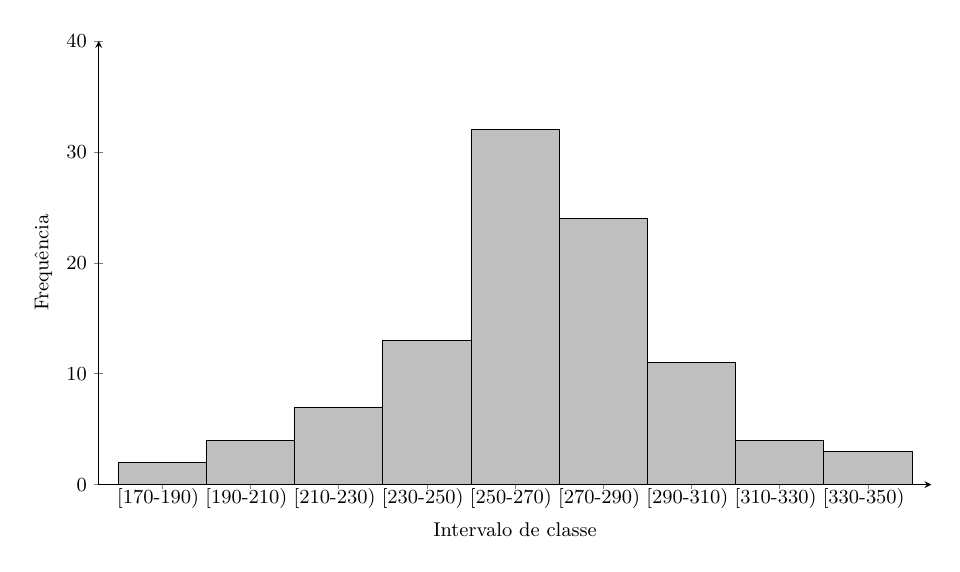
\begin{tikzpicture}[scale=0.8]
\centering
\scalefont{0.9}
\begin{axis}[  ybar,  ylabel=Frequência,  xlabel=Intervalo de classe,  ymin=0,  ymax=40,  axis lines=left,  enlarge x limits=0.09,  enlarge y limits=0, % aumenta 20%  
xtick=data,  xticklabels={[170-190),[190-210),[210-230),[230-250),[250-270),[270-290),[290-310),[310-330),[330-350)},  xticklabel style={rotate=0, anchor=east, xshift=0.7cm, yshift=-0.15cm},  bar width=1.4cm, width=10cm, x=0.07cm]
\addplot[fill=gray!50] coordinates {
    (180, 2)
    (200, 4)
    (220, 7)
    (240, 13)
    (260, 32)
    (280, 24)
    (300, 11)
    (320, 4)
    (340, 3)
    (340, 3)
    (340, 3)
    (340, 3)
};

\end{axis}
\end{tikzpicture}

\section*{Exercício 13}

\captionof{figure}{Gráfico de Dispersão do Peso versus Força de Resistência à Ruptura }
\label{tikz}
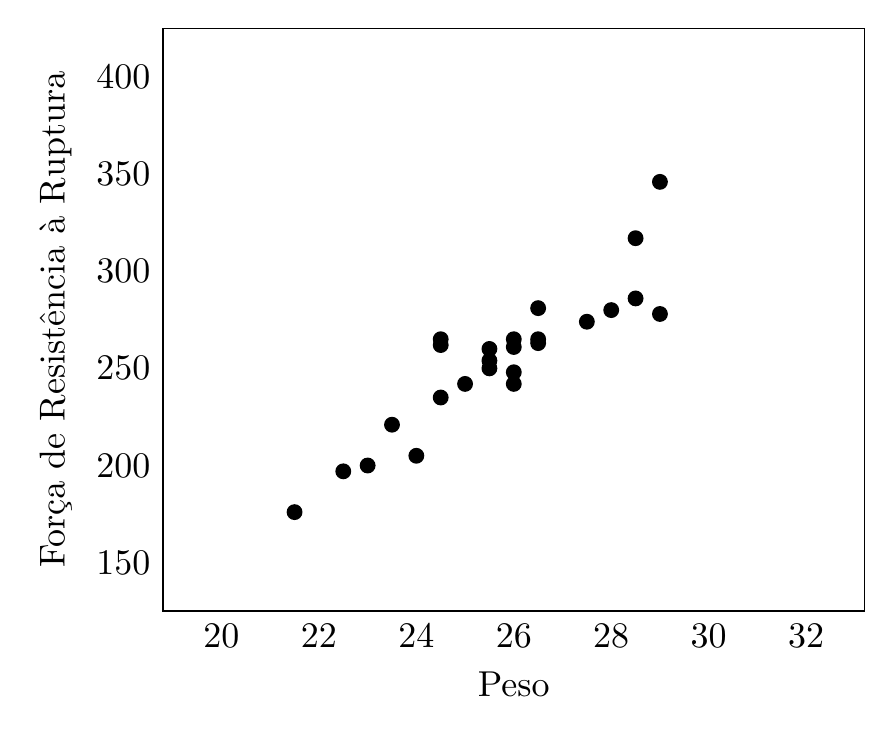
\begin{tikzpicture}[scale=1.3]
\centering

\begin{axis}[
  xlabel=Peso,
  ylabel=Força de Resistência à Ruptura,
  xmin=20, xmax=32,
  ymin=150, ymax=400,
  xtick={20,22,24,26,28,30,32},
  ytick={150,200,250,300,350,400},
  %%grid=both,
  enlargelimits=true,
      ytick style={draw=none},
    xtick style={draw=none},
]

\addplot[only marks] table {
x      y
26.00  265
22.50  197
29.00  346
28.00  280
26.50  265
23.00  200
23.50  221
24.50  265
26.00  261
29.00  278
24.00  205
28.50  286
28.50  317
26.00  242
25.50  254
24.50  235
21.50  176
24.50  262
26.00  248
25.50  250
26.50  263
27.50  274
25.00  242
25.50  260
26.50  281
};
\end{axis}
\end{tikzpicture}

Pode-se observar que está sendo formada uma núvem crescente de pontos próximos uns dos outros. \\
Calculando o coeficiente de correlação de Pearson chega-se no valor 0,9013, que indica que há uma correlação linear positiva. Ou seja, a medida em que o peso aumenta a força de resistência à ruptura também aumenta.




\end{document}

